\documentclass{sigchi}

% Arabic page numbers for submission.
% Remove this line to eliminate page numbers for the camera ready copy
\pagenumbering{arabic}

% Load basic packages
\usepackage{balance}  % to better equalize the last page
\usepackage{graphics} % for EPS, load graphicx instead 
\usepackage[T1]{fontenc}
\usepackage{txfonts}
\usepackage{mathptmx}
\usepackage[pdftex]{hyperref}
\usepackage{color}
\usepackage{booktabs}
\usepackage{textcomp}
% Some optional stuff you might like/need.
\usepackage{microtype} % Improved Tracking and Kerning
% \usepackage[all]{hypcap}  % Fixes bug in hyperref caption linking
\usepackage{ccicons}  % Cite your images correctly!
\usepackage[utf8]{inputenc} % for a UTF8 editor only

\usepackage{tikz}
\usepackage{pgfplots}
\pgfplotsset{compat=1.12}

\usepackage[inline]{enumitem}

% Paper metadata (use plain text, for PDF inclusion and later
% re-using, if desired).  Use \emtpyauthor when submitting for review
% so you remain anonymous.
\def\plaintitle{An Exploration of Automated Grading of Complex Assignments}
\def\plainauthor{First Author, Second Author, Third Author}
\def\emptyauthor{}
\def\plainkeywords{Automatic grading; ordinal regression; supervised
learning; active learning; text mining}

% llt: Define a global style for URLs, rather that the default one
\makeatletter
\def\url@leostyle{%
  \@ifundefined{selectfont}{
    \def\UrlFont{\sf}
  }{
    \def\UrlFont{\small\bf\ttfamily}
  }}
\makeatother
\urlstyle{leo}

% To make various LaTeX processors do the right thing with page size.
\def\pprw{8.5in}
\def\pprh{11in}
\special{papersize=\pprw,\pprh}
\setlength{\paperwidth}{\pprw}
\setlength{\paperheight}{\pprh}
\setlength{\pdfpagewidth}{\pprw}
\setlength{\pdfpageheight}{\pprh}

% Make sure hyperref comes last of your loaded packages, to give it a
% fighting chance of not being over-written, since its job is to
% redefine many LaTeX commands.
\definecolor{linkColor}{RGB}{6,125,233}
\hypersetup{%
  pdftitle={\plaintitle},
% Use \plainauthor for final version.
%  pdfauthor={\plainauthor},
  pdfauthor={\emptyauthor},
  pdfkeywords={\plainkeywords},
  bookmarksnumbered,
  pdfstartview={FitH},
  colorlinks,
  citecolor=black,
  filecolor=black,
  linkcolor=black,
  urlcolor=linkColor,
  breaklinks=true,
  hypertexnames=false
}

\begin{document}

\title{\plaintitle}

\numberofauthors{3}
\author{%
  \alignauthor{Leave Authors Anonymous\\
    \affaddr{for Submission}\\
    \affaddr{City, Country}\\
    \email{e-mail address}}\\
  \alignauthor{Leave Authors Anonymous\\
    \affaddr{for Submission}\\
    \affaddr{City, Country}\\
    \email{e-mail address}}\\
  \alignauthor{Leave Authors Anonymous\\
    \affaddr{for Submission}\\
    \affaddr{City, Country}\\
    \email{e-mail address}}\\
}

\maketitle

\begin{abstract}
Automated grading is essential for scaling up learning. In this paper, we
conduct the first systematic study of how to automate grading of a complex
assignment using a medical case assessment as a test case. We propose to
solve this problem using a supervised learning approach and introduce three
general complementary types of feature representations of such complex
assignments for use in supervised learning.  We first show with empirical
experiments that it is feasible to automate grading of such assignments
provided that the instructor can grade a number of examples. We further
study how to integrate an automated grader with human grading and propose
to frame the problem as learning to rank assignments to exploit pairwise
preference judgments and use NDPM as a measure for evaluation.  We then
propose a sequential pairwise online active learning strategy to minimize
the effort of human grading and optimize the collaboration of human graders
and an automated grader.  Experiment results show that this strategy is
indeed effective and can substantially human effort as compared with
randomly sampling assignments for manual grading.
\end{abstract}

\keywords{\plainkeywords}

\category{H.2.8}{Database Applications}{Data mining}

\def\ignore#1{}
\section{Introduction}

Information Technologies have been transforming education dramatically
recently, leading to the rapid growth of Massive Open Online Courses
(MOOCs), which have not only made education more affordable and scalable,
but also have huge potential to enable more effective personalized
learning.  Automatic grading technology has been a key component enabling
the success of MOOCs. Unfortunately, the
current technology for automatic grading is mostly limited to multiple-choice
questions, short answers~\cite{Brooks:2014:Powergrading,
Leacock:2003:CatH, Mitchell:2002:ICAA, Pulman:2005:EdAppsNLP,
Mohler:2009:EACL}, and simple essay scoring~\cite{Chen:2014:IRRODL,
Balfour:2013}, which makes it quite challenging for the current MOOCs to
provide sophisticated assignments for teaching complex concepts or skills
(e.g., critical thinking skills) since they cannot be easily graded in a
scalable way. A solution currently adopted to bypass this difficulty is to
use the calibrated peer review~\cite{Balfour:2013, Chen:2014:IRRODL,
Sandeen:2013, Suen:2014}.  However, there are systematic problems with this
approach: discrepancy between peer and instructor ratings, variation in
ratings over time by the same peer rater, inconsistency across exercises
for rating two works of similar quality, differences in rater stringency,
and random fluctuation of ratings of the same work under varied
conditions~\cite{Suen:2014}. Preliminary data from a recent attempt to use
this technique with veterinary students has also shown that peer reviews
have a distinct positive bias (vide infra) relative to an expert instructor
analysis~\cite{Ferguson:2014}. Thus, it is important to develop more
powerful automatic grading technology that can be applied to more
sophisticated exercises than those provided by the current MOOCs, which are
necessary in many education scenarios.

To automate grading of such a complex assignment, a natural idea is to use
supervised machine learning to learn from graded examples for automatically
assigning grades to ungraded assignments. As in other machine learning
applications, the general idea here is that if we can extract those
features from the assignments that can indicate the quality of an
assignment, a machine learning program would be able to pick up the
patterns of the features that can distinguish high-quality work from
low-quality work from a sample of graded assignments (i.e., ``training
data''), thus potentially assigning a grade automatically to an ungraded
assignment.

Although this idea is natural and appealing, there are many challenges and
questions that we must address before we can effectively deploy such a
technology in a real education environment, and a main goal of this paper
is to take a first step toward systematically addressing these questions.

\begin{enumerate}
  \item {\bf Feasibility:} How feasible is it to use machine learning to
    automate grading of a complex assignment?  What general features can we
    extract from assignments for automated grading? How effective are the
    state of the art machine learning approaches for automated grading? Are
    they sufficiently effective to be immediately useful in practice?

  \item {\bf Problem Formulation and Evaluation:}  How should we formulate
    the grading problem as a machine learning problem? There are at least
    two options. One is to frame it as a classification problem with the
    goal of classifying an assignment into one of the finite number of
    pre-defined grade levels based on a rubric. The other is to frame it as
    a ranking problem where the goal is to rank the assignments based on
    the quality without necessarily assigning a specific grade---human
    graders can then go through the ranked list to segment the assignments
    into different grade levels. How should we design evaluation metrics to
    measure the quality of the results of automated grading?

  \item {\bf Integration of Automated Grading and Human Grading:} How
    exactly should such an automated grader be integrated with instructor
    or TA grading? A more general question is: how can we optimize the
    collaboration of an imperfect automated grader with more reliable human
    graders? Intuitively, the optimization depends on a trade-off between
    the quality/reliability of grading and the amount of human effort
    required. But given an expected amount of human effort, what is the
    best way to have the automated grader to assist a person in grading?
    What is the best way to have a human grader help train the
    machine-learning based automated grader?
\end{enumerate}

We will study these questions using a particular type of complex
assignment that requires sophisticated critical thinking skills, i.e.,
medical case assessment. This kind of assignment is very important for
medical professional education. By studying how to automate grading
for medical assessment assignments, we can potentially enable medical
professional education to scale up---a much needed effort.
\ignore{
Traditional
veterinary curricula have usually consisted of didactic lectures for as
long as 3 years before entry into the clinic. In veterinary medicine, this
approach has been shown to result in an actual decline in critical thinking
skills~\cite{Herron:1992}. Therefore, to encourage self-awareness and
lifelong learning, didactic instruction should be supplemented by practice
with the process of information gathering and critical clinical thinking
associated with diagnosis of disease and selection of treatment. In her
book on critical thinking in clinical practice~\cite{Gambrill:2005},
Gambrill notes that evidence-based practice is rooted in a willingness to
recognize the intrinsic uncertainty of clinical decision-making.
%Not all clinicians are willing to acknowledge
%this uncertainty in their mission to help patients. This deficiency in
%training in critical clinical thinking is thus not unique to our veterinary
%curricula; in fact,
Furthermore, 
}
Not teaching clinicians about clinical uncertainty has been referred to as
``the greatest deficiency of medical education throughout the twentieth
century''~\cite{Djulbegovic:2004, Gambrill:2005}.
\ignore{
Evidence-based medicine (EBM) requires the skillset to develop answerable
questions relevant to a case, and to answer these questions with an honest
and open appraisal of research findings~\cite{Braddock:1999}.
Learning by doing is emphasized in EBM and evaluation of case
studies provides such practice. Instructors need to be prepared to provide
structure to the process together with timely feedback during practice in
order to be effective~\cite{Gambrill:2005}. }
However, implementing an instruction plan with an online education system
at large scale to teach clinical uncertainty in decision making raises many
significant challenges that must be solved, particularly challenges in
automatic evaluation of the case studies completed by the students, which
we address in this paper by leveraging information retrieval and machine
learning techniques.

To study the feasibility questions, we propose a general methodology for
designing three complementary types of feature representations of such
complex assignments, including token features, similarity features, and
selection features, and experiment with these features using ordinal
regression for predicting the grade levels in multiple dimensions of
rubrics. The token features are based on the term tokens extracted from an
assignment and they offer the most general representation and are robust in
practice. The similarity features are to capture the similarity between an
assignment and the solution provided by an instructor; the intuition is
that the higher the similarity is, the higher the grade should be.
Finally, the selection features are to quantify the accuracy of the
selection of relevant parts in a case description based on how well the
selected parts match the solutions (e.g., choosing to run the right
lab tests in a clinical case).  While it is generally beneficial to
manually design assignment-specific features, such features cannot be
generalized to work on other assignments; in this paper, we focus on
studying \emph{general} features that can be \emph{automatically computed}
on any semi-structured complex assignment, and aim at understanding their
effectiveness.

A practical challenge in studying our problem is the lack of a large set of
graded assignments which is needed both for training a machine learning
program and for validating the results of automated grading. This is partly
due to the fact that grading such assignments takes much human effort: the
very reason why we need to study automated grading for such assignments. In
our experiments, we used a data set of 107 student submissions for one
medical case assessment assignment that is available to us. While the data
set is small, we are able to observe statistically significant differences
in our experiments, thus it still allows us to draw meaningful conclusions
about different approaches to automated grading.

Our study with this data set shows that it is feasible to automate grading
of a complex assignment such as a medical case assessment using standard
machine learning approaches and the proposed three kinds of general
features provided the instructor can grade a small number of examples, but
the grading accuracy on different rubric categories varies substantially.

The results of our feasibility study reveal that there is a great deal of
variation in the grades given by instructors due to the inevitable
subjectivity of the rubrics. This suggests that it might be less effort
and more reliable for an instructor to make pairwise judgments between a
pair of assignments as opposed to assigning an exact numerical or letter
grade. Working on such pairwise preference judgments also makes it easy to
integrate non-expert judgments (such as peer grading) that might not be
reliable in the exact grades assigned but may include relatively reliable
preference judgments. Moreover, working on pairwise preferences naturally
``eliminates'' the need for normalizing numerical grades which might be
biased (e.g., some graders may be overly generous).

Given that we will attempt to obtain pairwise preferences as training
examples, it follows that we should frame the problem of automated grading
as to rank the ungraded assignments, as opposed to predict the exact grade
of an assignment. The ranking would be in descending order of quality (in
any rubric dimension or overall quality with consideration of multiple
dimensions), and a human grader can  then easily segment the list into any
desired grade levels.  In comparison with predicting exact grades, such a
ranking formulation also offers a natural way to engage humans in
validating and finalizing the grades.

For evaluation, although retrieval measures such as Mean Average Precision
(MAP) or normalized Discounted Cumulative Gain (nDCG) are commonly used for
evaluating a ranked list, we suggest that the Normalized Distance-based
Performance Measure (NDPM)~\cite{Yao:1995:JASIS} is a better measure for
our ranking problem since it can better handle many ties that inevitably
exist in our case.

In practice, an automated grader must be integrated with a human grader so
as to minimize the overall effort of the human grader while ensuring a
certain level of grading accuracy. There is an inherent trade-off here since
to increase the grading accuracy we would like to have as many training
examples (i.e., manually graded assignments) as possible, which, however,
would incur more human effort. To optimize human-machine collaboration and
enable a flexible trade-off between human effort and grading accuracy, we
propose the following sequential training process based on active machine
learning: 1) a human grader first grades a small number of assignments as
the initial training set (this could be either numeric or letter grades, or
pairwise judgments); 2) the machine would learn from the initial set,
and identify the next ``best'' example (i.e., assignment) to label and
present it for human to grade (where ``best'' here means that the example
is most valuable to help the automated grader improve its accuracy); 3)
a human would grade the nominated example to increase the size of the
training set by one; 4) the machine would learn from the augmented training
set and repeatedly present a new example for the human to grade until it
reaches a desired level of accuracy, at which point, the process stops and
the human grader would segment the final ranked list to generate grades for
all the assignments. Our experiment results show that such an active
learning process is much more effective than batch training.

As the first study of this new problem, our study is inevitably limited by
the size of the data set due to the unavailability of larger data sets; as
the automated grading technology matures for such assignments, we
anticipate to have much larger data sets available to further verify our
observations and conclusions.


\section{Related Work}

To the best of our knowledge, no previous work has studied how to automatically grade
a complex assignment such as a medical case assessment. However, our work
is related to multiple lines of existing work, which we briefly review below. 

Automated grading has been explored mostly for constrained question
types where the correct answer has a certain, well known form. Programming
assignments, for example, have long been a target for automatic
grading~\cite{Forsythe:1965:CACM, Helmick:2007:ITICSE} as their very medium
can easily be leveraged for providing ``yes'' or ``no'' feedback with
respect to programmatic correctness. For specific assignment types, more
sophisticated techniques like edit-distance of canonical representations
has been explored~\cite{Alur:2013:IJCAI}. Recent efforts have focused on
providing feedback to students about their programs by leveraging
structural similarities in the code itself to allow feedback to be provided
to many assignments at once that share particular
features~\cite{Nguyen:2014:WWW, Piech:2015:ICML}.

In this vein, clustering-based techniques have been applied to tools
designed to help instructors manually grade short-answer MOOC assignments
at scale by allowing them to assign grades to entire clusters of students
at once~\cite{Brooks:2014:Powergrading}. Hierarchical clustering methods
were applied in this work to allow the instructor to ``drill down'' as far
as he/she would like to assign grades and feedback to students. This method
is general and unsupervised but only explored the short-answer question
space, leaving more complex assignment outputs (like the outline-form case
assessments we study here).

Another approach would be to attempt to predict the grades explicitly. One
branch of work in this direction based on information extraction techniques
focuses on extracting fixed patterns from the answer: if the pattern (or
set of patterns) is matched, the question is correct, otherwise it receives
partial or no credit. Many methods require the manual construction of these
patterns~\cite{Mitchell:2002:ICAA, Leacock:2003:CatH}, while others attempt to
learn them from large training datasets~\cite{Pulman:2005:EdAppsNLP}. In either
case, the methods require strong supervision support to be effective.  Other
works take an unsupervised text-similarity approach and compare the student
answers with a gold standard answer using a wide variety of similarity
functions~\cite{Mohler:2009:EACL}.

Grading of long-form student answers has also been
explored~\cite{Balfour:2013}. In
\textsc{CarmelTC}~\cite{Rose:2003:HLT-NAACL-EDUC} a combination of topic
modeling and text classification approaches are taken to score student
essays. The system attempts to determine which ``key components'' have been
mentioned in each essay and uses this information to suggest to students
what components they may be missing. Approaches that purely use document
similarity metrics~\cite{Duwairi:2006:CHB} or purely supervised
classifiers~\cite{Larkey:1998:SIGIR} have been used for grading as well,
but the rubrics are not as complex as those required for medical case
assessment.

The task of predicting categorical labels with an implicit ranking (ordinal
variables) is often solved via ordinal regression
methods~\cite{McCullagh:1980}. These types of variables (and this
regression method) is very common in studies in the social sciences where
survey responses are often measured on scales such as (strongly disagree,
disagree, neutral, agree, strongly agree) which are called Likert
scales. Our work in predicting the grade labels for different dimensions of
an assignment's rubric can be seen as yet another application of ordinal
regression to the many applications already explored. Using machine
learning for optimizing ranking has been extensively in information
retrieval~\cite{Liu:2009}; our work explores an interesting novel
application of online active learning to automated grading where we are
interested in minimizing the training sample to label while maximizing the
ranking accuracy over a finite number of known test cases.  


\section{Medical Case Assignment}

Complex assignments inevitably vary across courses. As a first step toward
studying how to automate grading of such assignments, we  use a medical
case assignment in the veterinary medicine domain for our study. At a high
level, such an assignment represents a typical type of analysis assignment
where the students are given a case description with both an unstructured
text description as well as some structured data (e.g., lab test results),
and are asked to perform an analysis of the case. The analysis generally
involves 1) selecting relevant content from the case description, which can
be selected from both the text part and the structured data, 2) answering
questions with short textual answers, and 3) writing assessments in
natural language text.

More specifically, the case exercises were developed using
WhenKnowingMatters (WKM) web-based case formulation
software\footnote{\url{http://www.whenknowingmatters.com}} which
facilitates development and exchange of text-based cases while allowing
students to objectify their observations from a case and manipulate them in
an outline format around a suggested scaffold provided by the instructor.
The student's analysis is then rendered into a structured text format to
facilitate automatic grading.

\begin{figure*}[ht]
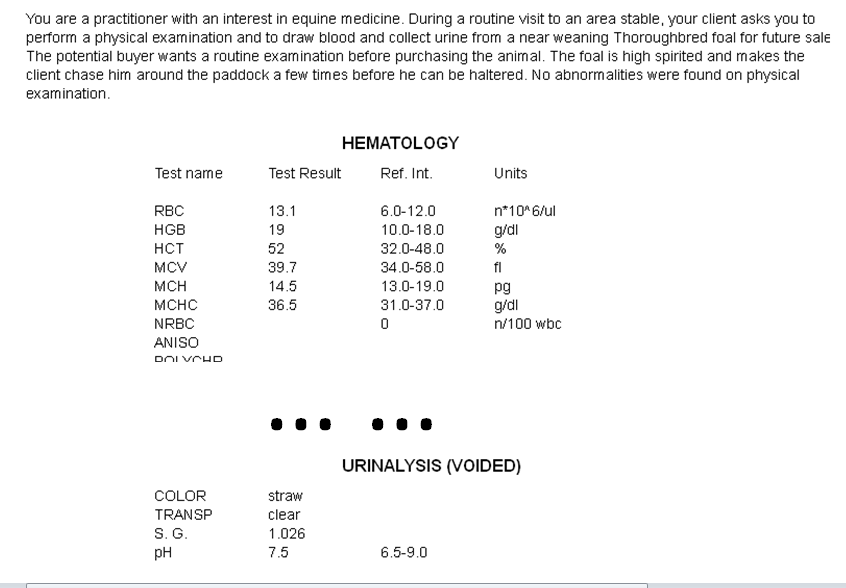
\includegraphics[scale=0.5]{case-desc-small.png}
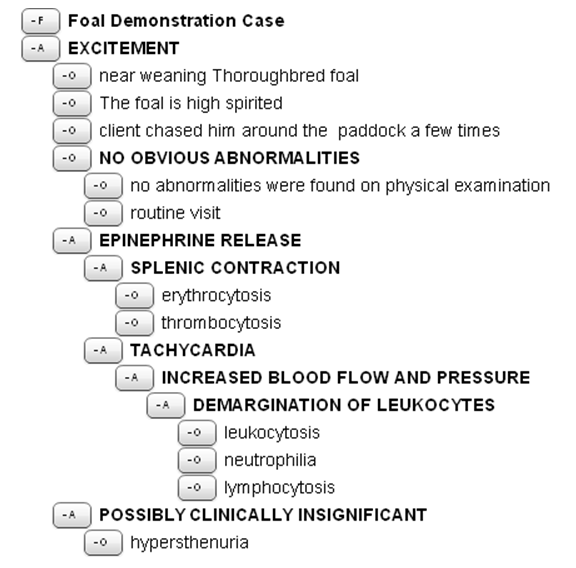
\includegraphics[scale=0.6]{student-work-small.png}
\caption{An example of case description (left) and student assessment (right)}
\label{fig:example}
\end{figure*}

Due to the lack of automated grading tools, the assignments are currently
graded manually. An assessment rubric designed prior to instruction was
used by the instructor to evaluate student performance on a subjective,
5-point scale (listed here in increasing order): novice, beginner,
competent, proficient, and expert. Rubric categories were related to
elements of critical thinking and communication:
\begin{enumerate}
\item {\bf Questions:} Developing relevant refining (or clarifying)
 questions to answer based upon an honest assessment of current knowledge
 base.
\item {\bf Answers:} Approach to seeking answers to developed
 questions; literature search, etc.
\item {\bf Quality:} Judgment of quality of information; awareness and
 application of standards of a discipline, bias detection including
 appropriate humility to detect one’s own potential bias, application of
 statistical concepts.
\item {\bf Analysis:} Analysis of an argument.
\item  {\bf Clarity:} Clarity and communication of thought; conciseness,
 grammar, spelling, elocution.
\item {\bf Application:} Application and understanding of appropriate
 disciplinary content.
\end{enumerate}

The instructor also created a ``gold standard" assessment for the
assignment case, which is available for the automated grading tool to use.

Figure~\ref{fig:example} shows an example of a very simple case and a typical
student answer. In the case description, the student can see a text
description of the case and a number of lab test results in the form of
structured data. The student assessment is seen to be a semi-structured
text with indented structures based on a scaffold provided by the
instructor. Multiple tags indicate different kinds of answers, including,
e.g., selected content from the original case description, selected lab
tests, and text input by the student reflecting his/her assessment.

Because of the complexity, automated grading of such an assignment is very
challenging. First, because of variations across different assignments, it
is almost impossible to learn from the grading results of one assignment to
automate grading of another, even though such an ``inter-assignment"
automated grading is ideal.  We thus focus on a more realistic setting of
attempting to automate the grading after the instructor has already graded
some assignments, which we may refer to as ``intra-assignment" automated
grading, which, strictly speaking, is actually semi-automatic grading.  Our
goal is thus to study whether and how we can leverage machine learning to
learn from the graded assignments to automatically predict the grades for
the rest of the ungraded assignments.


\section{Methods for Automated Grading}

In this section, we first provide a general discussion of how we might be able to use machine learning methods for automating the grading of complex assignments, and then present a general methodology for designing three complementary types of features for representing assignments, which are needed for supervised learning. 

\subsection{Unsupervised Learning}

Our first thought is to use unsupervised learning since it does not require any training data (i.e., graded assignments as examples).  In unsupervised learning, a model is built to describe some latent
structure of the data without considering any label information. Typical
examples of unsupervised methods include clustering and topic modeling.
Unsupervised methods have been applied to automated grading typically in
the form of clustering---the ``latent structure'' to be extracted are
groups of student submissions, which can then be collectively assigned a
single grade. Hierarchical clustering methods allow an instructor to
``drill down'' by dividing a single cluster into several smaller ones that
somehow capture differences within the same group. This method was
exploited to great effect by the power grading
project~\cite{Brooks:2014:Powergrading} to allow instructors to spend
significantly less time grading short answer questions.

However, this does not address the need to evaluate students along
different dimensions as occurs in rubric grading for complex assignments.  Because the method does
not consider the labels in learning the latent structure, the structure it
finds will tend to be general with no principled way of tuning it to
better describe the desired label outcomes. Furthermore, this strategy
also provides no guidance for the instructor in assigning the actual grade
value itself---while it aids in digesting the patterns that occur in the
data, the instructor is still on his/her own in deciphering what the grade
should be based on these patterns. With simple questions with more or less
one correct answer, this is not a problem---but when we attempt to address
more complex assignments that involve critical thinking and principled
analysis (for which there are many ``correct'' answers) this becomes much
more difficult and time consuming. 

\subsection{Supervised Learning}

Supervised learning is more useful in the sense that such an approach can directly 
assign a grade to an assignment though it requires some training data. In supervised learning, a model is built to predict the outcome (or label)
of a new example based on previous examples it has seen before (called the
training data). A critical component of this infrastructure is the
decomposition of examples into feature vectors---this decomposition enables
the use of algorithms for learning functions from these vectors to the
output labels desired. Typically, these feature vectors are either binary
or real-valued, and are often (but not always) in a high-dimensional space.
The performance of the learned function is directly tied to the features
used in the vector representation of the examples---poor features result
in low predictive capability due to the algorithm being unable to find
meaningful patterns in the examples. As such, these features are the most
critical component of any supervised learning approach. With a properly
defined set of features that are capable of capturing the salient patterns
in the training examples, the task can be given to any of a number of
state-of-the-art algorithms for learning appropriate predictive functions
that can be applied to yet-unseen data (the test data).

This scenario is applicable to an automated grading setup in which the
instructor labels a certain number of student assignments with a grade
which are then fed in to the algorithm to learn a predictive function that,
when applied to the unlabeled examples, provides a grade based on the
patterns extracted from the manually graded examples.

This supervised framework would allow instructors to learn a separate
predictor for each dimension in a rubric by simply changing the labels of
the training examples to reflect a different rubric dimension during
training. We will explore supervised learning approaches in this paper to
address our need for predicting different rubric dimensions instead of a
single overall grade. In such a setting, the grading problem has been
reduced to defining a set of features that characterize a student's
assignment along multiple dimensions.

\subsubsection{Defining Features of a Student Assignment}

The performance of a supervised learning approach is highly dependent on 
the effectiveness of the features fed into the learning program. Thus a main technical 
challenge we need to solve is how to design effective features for representing
an assignment. 

To address this challenge, we propose a general framework for defining features for complex
assignments such as the one we explore in this paper. The features we
propose are general in nature and thus should be applicable to any
assignment that is presented in a text-based, semi-structured response
form. We describe a set of feature classes and evaluate the performance of
these features on an example autograding task to evaluate their predictive
capacity. Our framework consists first of constructing a ``view'' of an
assignment and then defining features based on this view. The view chosen
for the assignment is critical in that it changes the way we may naturally
describe it and thus leads to the definition of distinct classes of
features distinguished by the view taken to derive them. We will explore
features by progressively taking views that make stronger assignment design
assumptions: while the features are still general, each view progressively
narrows the space of possible student response types.

The first class of features, which we call \textbf{token features}, are
generated by taking a view of the student response consistent with the
traditional ``bag of words'' approach common in information retrieval
contexts~\cite{Salton:1975:VSM}. In this view a document is decomposed into
a vector of count data that indicates the frequency of words within the
document. Two features are thus natural. The first type of feature would
indicate the number of occurrences of a given word in a student submission
(and is thus real-valued), and the second would indicate the presence or
absence of a word (and is thus binary-valued). These features would both
create a high-dimensional representation of the student submission, and are
motivated by an attempt to capture the difference in vocabulary between
assignments. This is often enough to capture whether the correct ideas are
mentioned without requiring extensive computation (features from this class
are trivial to compute for every student submission). Document
classification techniques typically operate in this kind of space.

The second class of features, which we call \textbf{similarity features},
are generated by characterizing a student submission by the ``distance''
from a gold standard (e.g., an assignment submission generated by the
instructor). With this view, features can be derived that strongly utilize
the structure of the assignment (e.g., how closely does the outline
structure of the student assignment match the outline structure of the
instructor assignment?)\ as well as features that loosely utilize or
completely ignore the structure of the assignment. Examples of features
that loosely utilize the assignment structure would be the similarity of
certain outline bullet types with the gold standard bullet types of the
same category. A bullet type in our examples could be ``observation''
(indicating something selected from the assignment text directly) or
``analysis'' (indicating original thoughts from the student). These
features require the assignment to be structured in such a way that this
information is easily extracted, but do not look so closely at the overall
structure of the outline itself. Ignoring the structure of the assignment,
features can be generated that indicate the overall similarity with the
gold standard. Document clustering techniques typically operate in this
kind of space, as well as retrieval functions in search
systems~\cite{Robertson:1994:SIGIR, Robertson:1996:TREC-3}.

The third class of features, which we call \textbf{selection features},
are generated by measuring concrete statistics about the selection of
bullet points compared to a gold standard. In some sense, these are similar
to the similarity features, but they differ in that they make a stronger
assumption about the assignment structure---namely, that students are
producing the exact same text that should occur in a similar section of the
gold standard. Examples of selection features would be precision (what
fraction of the bullets selected by the student also appear in the gold
standard?)\ and recall (what fraction of bullets selected in the gold
standard were also selected by the student?).

\subsection{Active Learning}
One critical problem in the supervised learning setting is the selection
of a training set. If a non-representative training set is selected, the
algorithm has no opportunity to learn the features that distinguish the
excellent submissions from the ordinary submissions. Unfortunately, the
traditional supervised learning setting offers no principled mechanism for
picking which training set to use---it just assumes one exists a priori.

Active learning methods~\cite{Settles:2012} bridge this gap by providing a
mechanism for selecting relevant training examples designed to maximally
improve the performance of an existing model. This setting is very relevant
for an autograding setup, where the system should ideally ask the
instructor to grade a \emph{specific} set of examples, rather than forcing
the instructor to find good representative examples on his/her own. This
process can be iterative: the system can learn from the first batch of
examples graded by the instructor, and then request him/her to grade a
second batch, which is used to incrementally improve the learned model.
This should, in principle, reduce the amount of time an instructor would
have to spend grading to obtain a certain performance threshold for the
grade predictor.

\subsection{Combined Methods for Complete Grading Support}

A comprehensive system can then be designed that leverages all three of
these perspectives: unsupervised, (semi-) supervised, and active learning.
We can first apply an unsupervised learning technique to group the student
assignment data into rough categories. Then, a set of student submissions
can be sampled from these distinct categories, resulting in a collection of
submissions that are in some sense different from one another---these
examples are then labeled by the instructor and used as the starting point
for an active learning method: we can learn a supervised classifier using
the now labeled data, use this classifier to separate the remaining
unlabeled training data, sample more documents for the instructor to label,
and continue in an iterative fashion until either a fixed evaluation
criteria is met, or a certain number of submissions have been labeled.
Such a combined method would attempt to {\bf optimize the collaboration of
human graders and the automated grading tool}  so that we can leverage the
best of each.



\section{Automated Grading as Ranking Assignments}

\subsection{Motivation}

Some of the results from our feasibility study using ordinal regression raise
 the question whether framing the problem of automated grading as
ordinal regression is appropriate. Indeed, as we will discuss, it appears
to be more advantageous to frame the problem as one of ranking
the ungraded assignments, which a human grader can segment  into
any desired grade levels. 

Specifically, as we observed in
Tables~\ref{table:feature-comb}~and~\ref{table:feature-comb-clar}, outright
prediction of an ordinal grade can be very challenging due to the highly
concentrated nature of the dataset labels (see
Table~\ref{table:grade-stats}). The vast majority of grade information
available for the grade prediction task is centered around the mean,
leaving very little information in the tails for a supervised learner to
extract patterns from. (In some cases, for example, there are as few as one
example for the highest and lowest ordinal grade values). The result is
noisy output that may be inappropriate for using directly. However, it is
worth noting that ordinal grade prediction is a hard problem, even for
humans: a previous study suggests disagreement rates around $44\%$ for
short answer grading~\cite{Mohler:2009:EACL}. We suspect that this only
becomes larger as assignments become more complex and difficult to grade,
which makes the task of outright label prediction much more difficult for
the machine as well.

Thus  an alternative, and more reasonable approach may be to produce a ranked list of
assignments from best to worst. Annotators are typically more consistent at
providing judgments of the form ``is $a$ better than $b$?''\ than ``on a
scale from 1--5, how good is $a$?''~\cite{Callison-Burch:2007:WMT}, so it
is reasonable to suspect that a machine learning model could achieve better
results when trained using such pairwise judgments. If a system can provide
a good ranking of assignments, an instructor simply needs to assign
``cutoff'' points in this ranking to determine grades. This simplifies the
learning problem from attempting to predict an ordinal label for a specific
assignment to assigning a ranking to a set of assignments. This is a well
studied area in information retrieval called ``learning to
rank''~\cite{Joachims:2002:KDD, Liu:2009}, and there are a wide variety of methods
available that one can use to learn a ranking function for documents given
a set of available features.  

One particular method that we will explore is ......  Before we explore the efficacy of such an approach, however, we must first
redefine some measure by which we can measure performance. Because the
system is no longer predicting a rating for each assignment, we cannot use
MAE as before.

\subsection{Evaluating Ranking-based Grading Systems}
Our goal is to produce a ranking of student assignments that is consistent
with instructor evaluation. One way of framing this problem is to compare
the ranking produced by the system to the ranking produced by the
instructor (which we'll call the ``reference ranking''). A system's ranking
can then be evaluated using some measure of correlation between the two
rankings. We note a preference for metrics that take into account the
\emph{entire} ranked list---this contrasts with most of the preferred
measures in information retrieval evaluation which typically place heavier
emphasis on the top-ranked elements. While this makes sense in a search
context, our goal is to produce an exhaustive ranking of the assignments,
so we focus on these types of measures.

Measures for rank correlation are plentiful. Perhaps the most commonly
used metrics are Kendall's $\tau$ or Spearman's $\rho$ (which have been
found to be highly correlated in practice~\cite{Shani:2011:Springer}; thus,
we present only one for illustration). Kendall's $\tau$ can be formulated
as
\[
    \tau = \frac{n_c - n_d}{\frac{1}{2} n (n-1)},
\]
where $n_c$ is the number of \emph{concordant pairs}, and $n_d$ is the number
of \emph{discordant pairs}, and $n$ is the number of items ranked. To
compute $n_c$ and $n_d$, one considers all pairs $(x_i, y_i)$ and $(x_j,
y_j)$ (that is, pairs of tuples) of assigned rankings in the system ranking
$X$ and the reference ranking $Y$ (the denominator is simply the number of
such pairs). A pair is \emph{concordant} if the ordering of the items $i$
and $j$ in $X$ and $Y$ is consistent---in other words, if $(x_i < x_j)
\land (y_i < y_j)$ or $(x_i > x_j) \land (y_i > y_j)$.  A pair is
\emph{discordant} if the ordering of items in the two lists is
inconsistent---in other words, if $(x_i < x_j) \land (y_i > y_j)$ or $(x_i
> x_j) \land (y_i < y_j)$. This is then a correlation measure, with values
bounded in $[-1, 1]$, with $1$ indicating a perfect correlation and $-1$
indicating inverse correlation.

One of the assumptions Kendall's $\tau$ makes is that there are no ties in
ranks. However, in a realistic grading scenario based on rubrics we expect
many ties. Fortunately, there is a variation of Kendall's $\tau$, denoted
as $\tau_b$, that accounts for ties in the rankings. This is formulated as
\[
    \tau_b = \frac{n_c - n_d}{\sqrt{(n_c + n_d + t_x)(n_c + n_d + t_y)}}
\]
where $t_x$ is the number of pairs that were tied on \emph{only} their
ranking from $X$, and $t_y$ is the number of pairs that were tied on
\emph{only} their ranking from $Y$.

This may, at first glance then, seem like a good measure to use, but it is
not without its problems. Despite taking into account ties in the rankings,
it may still penalize a system for re-ordering items that were tied in the
reference ranking---in other words, we may be penalized for not correctly
identifying elements who are tied in the reference ranking. Consider a
simple example: suppose the ranking proposed by a system is $X =
(1,2,3,4,5,6)$ but the reference ranking is $Y = (1,1,2,2,3,4)$.
Intuitively, the system made no real mistakes in that no pair where the
reference ranking asserted an is in the wrong order in $X$. However, we'll
see that $\tau_b \approx 0.9309$, indicating that the system did not achieve
perfect correlation.

To address this issue, Yao~\cite{Yao:1995:JASIS} proposed the normalized
distance-based performance measure (NDPM), which computes a distance
between two rankings that is insensitive to a system's reordering of tied
elements in the reference ranking. NDPM is computed as
\[
    NDPM = \frac{2n_d + t_x}{2(n_c + n_d + t_x)}.
\]
Note that this is a \emph{distance} measure, so a value of $0$ would
indicate a perfect ranking. Indeed, if we compute NDPM for the example
rankings above, we achieve this result. Thus, we feel that NDPM is perhaps
the most appropriate measure for evaluating automatic grading systems that
produce an ordering of assignments as their output.

\section{Efficiently Utilizing Human Judgments with Active Learning}
As in all supervised learning approaches, 
the accuracy of  the automated grader based on learning to rank. depends
on the quantity and quality of the training examples available for the 
learner to use. Ideally, we would like human graders to provide
 as many graded examples as possible, but this would
reduce the benefit of an automated grader. Indeed,
if a human grader completes grading all the assignments,
there would be no need for the automated grader!
However, if there are insufficient training examples 
to learn from, the automated grader migh have a low accuracy,
which would further require more human effort on 
``post-editing" the grading results of the automated grader. 
Thus there is clearly a complicated tradeoff between
the effort of manual grading and the utility of the trained
 grader that may have to be empirically optimized in an application-specific way.

However, it is very clear that if we ask human graders to grade
a certain amount of assignments, we would like the
graded assignments to be as useful to the automated grader as possible.
Just randomly selecting a sample of assignments for manual grading
is not the best way. 
\ignore{
A serious drawback of the supervised learning approach is the lack
of early feedback in the instructor--machine collaboration. In the
supervised approach, a model is learned on some subset of the assignments
to predict the grades of the remaining assignments, but the process of
selecting a subset of assignments for grading is not guided. It is possible
that randomly selecting assignments to grade results in mostly redundant
information being given to the grading model. Instead, }
A natural solution to this problem is to employ 
active learning to allow the machine learning model to
guide the instructor in providing the supervision to make the most
effective use of his/her effort.

Building on these observations, we thus propose the following ``pairwise active
learning to rank'' model for automatic grading, which will employ the
following process where $k_1$ is a parameter that can be empirically set:
\begin{enumerate*}[label=\itshape(\arabic*)\upshape]
  \item Ask the instructor for comparative judgments on $k_1$ pairs of
    assignments,

  \item Learn a model using a learning-to-rank approach on the available
    pairwise judgments\label{al:learn-model-step},

  \item Apply the model to all remaining unjudged pairs,

  \item Select an unjudged pair to present to the instructor for
    judgment\label{al:select-training-step}, and

  \item Go to step~\ref{al:learn-model-step}.
\end{enumerate*}
Instantiations of this general approach will differ mainly in
steps~\ref{al:learn-model-step}~and~\ref{al:select-training-step}.

% subsection heading removed for space...
%\subsection{Experiments}

To study whether our proposed active learning approach better utilizes
human judgments during the grading process, we performed the following
experiment. We took our assignments and assigned each a ``composite
score'', computed as the average of their ordinal score for each of the six
rubric dimensions. Our task is then to learn a ranking that is consistent
with the ranking produced by these composite scores while simultaneously
\emph{minimizing instructor effort} in labeling.

We first transform the $n = 107$ assignments into $\frac{1}{2}n(n-1) =
5671$ assignment \emph{pairs} $(x_i, x_j)$ with corresponding labels
$y_{ij} \in \{+1, -1\}$ indicating whether $x_i$ should be ranked above or
below $x_j$ in the ranking. Ties were broken arbitrarily by assignment id.
The supervision given by the instructor is then to indicate a preference
for ranking $x_i$ relative to $x_j$.

Following the process laid out in the beginning of the section, we first
start with $k_1 = 10$ random pairs selected from the transformed data and
ask for labels from the instructor. We then learn the model, compute the
NDPM for the ranking produced by the model for all $n$ assignments, and
then ask for additional supervision by selecting the unlabeled assignment
pair whose distance from the decision boundary for the model is lowest
(this is a known, simple approach to uncertainty
sampling~\cite{Settles:2012}) and repeat the training/evaluation loop. Our
particular model choice was a linear SVM provided through the \textsc{MeTA}
toolkit.

We compare this active learning scenario with a random learning baseline,
which is the exact same process as above, but instead of selecting the most
uncertain pair in the unlabeled data we select one uniformly at random.
This will allow us to see whether the uncertainty sampling approach is
truly helping to guide the learning process to make more efficient
supervision choices or not.

\begin{figure}
  \begin{center}
   \begin{tikzpicture}[scale=0.9]
    \begin{axis}[xlabel={human-labeled pairs},ylabel={NDPM}, xmax=500,
      legend style={font=\small}]

      \addplot+[color=red, each nth point={10}, filter discard
          warning=false, mark=triangle, error bars/.cd, y dir=both, y explicit]
        table [x=training-size, y=AVG-NDPM, y error=std-deviation, col
            sep=comma] {data/random-learning.csv};

      \addplot+[color=blue, each nth point={10}, filter discard
          warning=false, mark=x, error bars/.cd, y dir=both, y explicit]
        table [x=training-size, y=AVG-NDPM, y error=std-deviation, col
          sep=comma] {data/active-learning.csv};

%      \addplot[mark=none, color=green]
%        coordinates {(0, 0.344637) (500, 0.344637)};

      \legend{Random learning, Active learning, BM25 similarity}
    \end{axis}
  \end{tikzpicture}
  \caption{A comparison between a randomized learning solution and an
  active learning solution to the grading-as-ranking problem. Reported is
  the average NDPM (lower is better) over 5 runs, with error bars indicating
  one standard deviation.}
  \label{fig:active-learning}
\vskip-10pt
  \end{center}
\end{figure}

Our results are summarized in Figure~\ref{fig:active-learning}. Recall that
a NDPM value of $0.3$ indicates that a system ranking was 30\% of the
maximal achievable distance away from the reference ranking. We can see
that even at a small fraction of all of the assignment pairs, the active
learning approach (blue line) is able to achieve better NDPM than simply
learning at random (red line). This is consistent with our hypothesis that
active learning as part of an automatic grading system can make more
effective use of an instructor's time than a purely passive supervised
approach.

How much instructor effort goes in to judging 200 assignment pairs? This
may initially seem like a lot, but each pair is not labeled in
isolation---labeling many pairs will inevitably include assignments that
have already been seen before. These familiar assignments make providing a
pairwise judgment faster than it would be if done ``cold''. In general, it
is also reasonable to assume that the effort involved in simply saying
whether assignment $a$ is better than assignment $b$ is lower than having
to consult a rubric to assign an actual point (or letter) value. It is
important, however, to ensure that providing a pairwise judgment takes as
little effort as possible relative to assigning a numeric or letter grade.
An interesting future direction is then to design an interactive system
that attempts to further drive the cost of providing judgments down.



\section{Conclusions and Future Work}

Automated grading of complex assignments is necessary for scaling up learning without compromising 
effectiveness of learning. Using a data set of medical case assessment assignments, 
 we conducted the first systematic study of how we might be able to use machine learning to automate grading
of such a complex assignment. Our study has led to several contributions. 

First, we have experimentally shown the feasibility of using
supervised learning techniques for automated grading of medical case assignments under certain conditions
provided that the instructor can manually label a number of the
assignments to serve as a training set. In particular,  an ordinal regression
method can be applied to the data with results that consistently outperform
the majority-label baseline in terms of mean absolute error.

Second, we proposed a general framework for the development of three complementary types of 
representative
features for student submissions (i.e., token features, similarity features, and selection features) ---while we applied these features to our
specific task of medical case analysis grading, these feature types (and
generation framework) are general and should apply to the grading of any
complex assignment.

Third, we proposed to frame the problem of automated grading as a ranking 
problem, which can more naturally assist human graders to validate
and finalize grades of ungraded assignments and learn from pairwise
preference judgments that can be potentially created more reliably by human
graders including through peer grading. We also suggested
NDPM as potentially a better measure for this ranking task than other measures due to its superiority in handling many tied cases. 

Finally, we proposed an iterative procedure of online active learning to rank to efficiently
utilize human judgments, and thus optimizing the collaboration between human graders and
  the automated grader. Experiment results confirm the efficiency of this procedure
which can substantially save human effort as compared with randomly choosing
sample assignments for humans to grade. 

A major limitation of our study is the limited size of the data set. 
This is partly due to the fact that such complex assignments currently can only be graded
by human graders. In the future, we hope to deploy our automated grading tools
to help scale up such courses to enable more students to participate, which in turn, would
help collecting more data for experiments. 

\ignore{
 While the problem is not completely solved, this method shows promise. We
believe that with more work, complex outline-based assignments such as the
medical case assignments we study here can be autograded sufficiently well
across many different rubric dimensions. We expect our findings to be
applied to the veterinary medicine class from which this data was obtained.
The automation provided by our method will enable faster feedback to
students than was previously possible, and we will continue to work on
reducing the method's error rate on the other rubric dimensions.
%
Moving forward, we should consider new feature instantiations that follow
(or extend upon) our feature generation framework in order to better
capture the patterns we require for grading different dimensions such as
``clarity''. One example might be spelling/grammar mistakes, which could in
principle be extracted by taking a token-based view. Novel features not
explored here could also extend to evaluating the quality of references
within the assignment.
%
We also believe that an active learning approach should be effective for
automating the training set selection of our method, which is currently a
weakness of the proposed solution. We would like to address the
effectiveness of an active learning-based automatic grading approach.
Another limitation of our study is that the data set used for evaluation is small.
}



Another direction that remains unexplored is feedback: how could such a
system give more detailed feedback to students beyond just their ordinal
rating along a rubric dimension? Currently, peer grading approaches have
an advantage in this sense, as your peers can suggest to you corrections
or point out specific mistakes that you made. It is worth investigating
whether or not we can generate ``explanatory reports'' of grading results
when using a supervised learning approach such as this.


\section{Acknowledgments}

Anonymized for blind reviewing.

\balance

\bibliographystyle{SIGCHI-Reference-Format}
\bibliography{auto-grading}
\end{document}
